% Pre Thesis 1 (P1) report
% Structure follows "P1 Content": Chapter 1 and Chapter 2 (graded), the optional
% Chapter 3 (Preliminary Design and Planning) and the Conclusion as Chapter 4.
% Compiles with pdfLaTeX, XeLaTeX or Tectonic. On Overleaf: upload this whole folder
% (WiFi.tex, frontmatter/, chapters/, signatures/) and press Recompile.
%
% File layout
%   WiFi.tex                         preamble, names to fill in, order of the parts
%   frontmatter/titlepage.tex        title page
%   frontmatter/declaration.tex      declaration and student signatures
%   frontmatter/approval.tex         examining committee
%   frontmatter/abstract.tex         abstract and keywords
%   frontmatter/nomenclature.tex     abbreviations
%   chapters/01_introduction.tex     1.1 to 1.5
%   chapters/02_literature_review.tex  2.1 to 2.4
%   chapters/03_preliminary_design.tex 3.1 to 3.8
%   chapters/04_conclusion.tex       conclusion
%   (bibliography)                   at the end of this file

\documentclass[12pt,a4paper]{report}

\usepackage[T1]{fontenc}
\usepackage[utf8]{inputenc}
\usepackage[a4paper,left=1.25in,right=1in,top=1in,bottom=1in]{geometry}
\usepackage{setspace}
\usepackage{graphicx}
\usepackage{booktabs}
\usepackage{longtable}
\usepackage{array}
\usepackage{enumitem}
\usepackage{tikz}
\usetikzlibrary{positioning,arrows.meta,fit,calc,shapes.geometric}
\usepackage[hidelinks]{hyperref}

% ---------------------------------------------------------------------------
% FILL THESE IN. Everything in [square brackets] below is a placeholder.
% ---------------------------------------------------------------------------
\newcommand{\thesistitle}{Device-Free Human Presence and Movement Detection Using Channel State Information from Commodity Wi-Fi Devices}
\newcommand{\studentA}{Kamrul Islam Kamran}
\newcommand{\idA}{24341149}
\newcommand{\studentB}{Adiyan Abdur Rahman}
\newcommand{\idB}{22241103}
\newcommand{\studentC}{Ahnaf Awsaf}
\newcommand{\idC}{22201408}
% Signature images, cropped copies of the PNGs in the project folder.
% Keep each one on the same letter as the student it belongs to.
\newcommand{\sigA}{signatures/kamran}
\newcommand{\sigB}{signatures/adiyan}
\newcommand{\sigC}{signatures/awsaf}
\newcommand{\supervisor}{Sheikh Araf Noshin}
\newcommand{\supervisortitle}{[Designation]}
\newcommand{\sigSupervisor}{signatures/araf_noshin}
\newcommand{\coordinator}{Md. Golam Rabiul Alam}
\newcommand{\coordinatortitle}{Professor}
\newcommand{\head}{Sadia Hamid Kazi}
\newcommand{\headtitle}{Chairperson and Associate Professor}
\newcommand{\department}{Department of Computer Science and Engineering}
\newcommand{\university}{Brac University}
\newcommand{\degree}{B.Sc. in Computer Science and Engineering}
\newcommand{\semester}{[Semester, Year]}
\newcommand{\submissionmonth}{October 2026}
\newcommand{\submissionyear}{2026}
% ---------------------------------------------------------------------------

% \signatureblock{name}{id}{signature image}
\newcommand{\signatureblock}[3]{%
  \begin{minipage}[t]{0.45\textwidth}\centering
    % The image is used only if the file is there; without it the line stays blank.
    \IfFileExists{#3.png}{%
      \vspace{0.5cm}
      \includegraphics[height=1.1cm,width=0.8\linewidth,keepaspectratio]{#3}\\[-2pt]}{\vspace{1.6cm}}
    \rule{0.85\linewidth}{0.4pt}\\[4pt]
    #1\\[2pt]
    #2
  \end{minipage}}

% \committee[signature image]{role}{member or chair}{name}{designation}
\newcommand{\committee}[5][]{%
  \noindent\textbf{#2}\\
  (#3)\par
  \IfFileExists{#1.png}{\vspace{-0.1cm}}{\vspace{1.1cm}}
  \begin{flushright}
  \begin{minipage}{0.62\textwidth}\centering
    \IfFileExists{#1.png}{%
      \includegraphics[height=1.2cm,width=0.7\linewidth,keepaspectratio]{#1}\\[-4pt]}{}
    \rule{0.9\linewidth}{0.4pt}\\[4pt]
    #4\\[4pt]
    #5\\
    \department\\
    \university
  \end{minipage}
  \end{flushright}
  \vspace{0.6cm}}

\newcolumntype{L}[1]{>{\raggedright\arraybackslash}p{#1}}
\setlength{\emergencystretch}{1em}

% Stick figure for the use case diagram: \actor{name}{x,y}{label}
% defines the coordinates (name-w) and (name-e) for the association lines.
\newcommand{\actor}[3]{%
  \begin{scope}[shift={(#2)}]
    \draw (0,0.55) circle (0.18);
    \draw (0,0.37) -- (0,-0.15);
    \draw (-0.3,0.2) -- (0.3,0.2);
    \draw (0,-0.15) -- (-0.25,-0.6);
    \draw (0,-0.15) -- (0.25,-0.6);
    \node[font=\footnotesize, align=center] at (0,-0.95) {#3};
    \coordinate (#1-w) at (-0.45,0.1);
    \coordinate (#1-e) at (0.45,0.1);
  \end{scope}}

\begin{document}

% ============================ Front matter ==================================
% No page anchor on the title page: it is an unnumbered page 1 and would clash
% with page 1 of Chapter 1 in the PDF links.
\hypersetup{pageanchor=false}
\begin{titlepage}
\centering
{\large Pre Thesis 1 Report\par}
\vspace{1.5cm}
{\LARGE\bfseries \thesistitle\par}
\vspace{1.5cm}
{\large by\par}
\vspace{0.6cm}
{\large
\studentA\\ \idA\\[4pt]
\studentB\\ \idB\\[4pt]
\studentC\\ \idC\par}
\vspace{1.5cm}
{A thesis submitted to the \department\\
in partial fulfillment of the requirements for the degree of\\
\degree\par}
\vfill
{\department\\
\university\\
\submissionmonth.\par}
\vspace{1cm}
{\copyright\ \submissionyear. \university\\
All rights reserved.\par}
\end{titlepage}

\hypersetup{pageanchor=true}

\pagenumbering{roman}
\onehalfspacing

\chapter*{Declaration}
\addcontentsline{toc}{chapter}{Declaration}
It is hereby declared that
\begin{enumerate}
  \item The thesis submitted is our own original work while completing degree at \university.
  \item The thesis does not contain material previously published or written by a third party, except where this is appropriately cited through full and accurate referencing.
  \item The thesis does not contain material which has been accepted, or submitted, for any other degree or diploma at a university or other institution.
  \item We have acknowledged all main sources of help.
\end{enumerate}

\vspace{0.5cm}
\noindent\textbf{Student's Full Name \& Signature:}

\begin{center}
\signatureblock{\studentA}{\idA}{\sigA}\hfill
\signatureblock{\studentB}{\idB}{\sigB}

\signatureblock{\studentC}{\idC}{\sigC}
\end{center}

\chapter*{Approval}
\addcontentsline{toc}{chapter}{Approval}
The thesis titled ``\thesistitle'' submitted by
\begin{enumerate}
  \item \studentA\ (\idA)
  \item \studentB\ (\idB)
  \item \studentC\ (\idC)
\end{enumerate}
of \semester\ has been accepted as satisfactory in partial fulfillment of the requirement for the degree of \degree.

\vspace{0.4cm}
\noindent\textbf{Examining Committee:}
\vspace{0.4cm}

\committee[\sigSupervisor]{Supervisor:}{Member}{\supervisor}{\supervisortitle}
\committee{Thesis Coordinator:}{Member}{\coordinator}{\coordinatortitle}
\committee{Head of Department:}{Chair}{\head}{\headtitle}

\chapter*{Abstract}
\addcontentsline{toc}{chapter}{Abstract}
Wi-Fi signals fill almost every indoor space, and a person who stands or moves in that space changes how those signals travel from a transmitter to a receiver. The Channel State Information (CSI) reported by a Wi-Fi receiver records this change for every subcarrier of the signal, so an ordinary Wi-Fi link can work as a sensor that needs no camera and no wearable device. Over the last decade, researchers have used CSI to detect motion, to notice people behind walls, to recognise daily activities, to detect falls and to measure breathing. Most of these systems, however, were built on a few specific network cards and routers with several antennas, and many of their reported accuracies were measured in the same environment in which the system was set up or trained.

This research asks how much of this sensing ability can be reached with ordinary commodity Wi-Fi devices that many people already have access to, without any special radio equipment. We review nineteen works on Wi-Fi based presence detection, through-the-wall detection, activity recognition, fall detection and vital sign monitoring, compare their hardware, methods and reported results, and identify the gaps that remain. Based on this review we propose a system with one commodity Wi-Fi transmitter and three commodity Wi-Fi receivers that detects presence and movement, gives a coarse estimate of where the movement is, and is evaluated on recording sessions that were not used for training, so that the reported accuracy is not optimistic.

\vspace{0.5cm}
\noindent\textbf{Keywords:} Wi-Fi Sensing, Channel State Information, Device-Free Sensing, Human Presence Detection, Motion Detection, Commodity Wi-Fi Devices, Internet of Things


% \addcontentsline comes first so that the entry points to the first page of each list
\renewcommand{\contentsname}{Table of Contents}
\clearpage
\addcontentsline{toc}{chapter}{Table of Contents}
\tableofcontents

\clearpage
\addcontentsline{toc}{chapter}{List of Figures}
\listoffigures

\clearpage
\addcontentsline{toc}{chapter}{List of Tables}
\listoftables

\chapter*{Nomenclature}
\addcontentsline{toc}{chapter}{Nomenclature}
The next list describes several symbols \& abbreviations that will be later used within the body of the document.

\begin{description}[leftmargin=3cm,style=sameline,itemsep=2pt]
  \item[AP] Access Point
  \item[BiLSTM] Bidirectional Long Short-Term Memory
  \item[CNN] Convolutional Neural Network
  \item[CSI] Channel State Information
  \item[DBSCAN] Density-Based Spatial Clustering of Applications with Noise
  \item[DWT] Discrete Wavelet Transform
  \item[GRU] Gated Recurrent Unit
  \item[HMM] Hidden Markov Model
  \item[IoT] Internet of Things
  \item[LoS] Line of Sight
  \item[LSTM] Long Short-Term Memory
  \item[MIMO] Multiple-Input Multiple-Output
  \item[MLP] Multilayer Perceptron
  \item[NIC] Network Interface Card
  \item[OFDM] Orthogonal Frequency Division Multiplexing
  \item[PCA] Principal Component Analysis
  \item[PIR] Passive Infrared
  \item[RSS] Received Signal Strength
  \item[RX] Receiver
  \item[SVM] Support Vector Machine
  \item[TTW] Through-The-Wall
  \item[TX] Transmitter
\end{description}


\clearpage
\pagenumbering{arabic}

% ============================ Chapters ======================================
\chapter{Introduction}

\section{Background}
Wi-Fi was designed to carry data, but the radio signal that carries the data also carries information about the room it passes through. A signal sent by a transmitter does not reach the receiver along one straight line only. It also arrives after bouncing off walls, furniture and people, and the receiver gets the sum of all these copies. This is called multipath propagation. When the room is empty and nothing moves, the paths stay the same and the received signal is almost constant. When a person walks, sits down, falls or even breathes, some of the paths become longer or shorter, the copies add up differently, and the received signal changes over time. Reading these changes makes it possible to sense people without asking them to carry any device, which is why this field is called device-free or passive sensing.

Early device-free systems used the Received Signal Strength (RSS), a single number per packet that describes the overall power of the signal. RSS is easy to obtain on any device, but it is coarse and it varies even in a static room, so slow or small movements are easily hidden in its own noise \cite{fimd,pads}. Modern Wi-Fi uses Orthogonal Frequency Division Multiplexing (OFDM), which splits the channel into many narrow subcarriers. For each received packet, the receiver estimates the amplitude and the phase of every subcarrier. This estimate is the Channel State Information (CSI). Because CSI describes the channel at the level of single subcarriers and not as one total power value, it is stable in a static environment and at the same time sensitive to movement, and it captures small-scale fading patterns that RSS cannot show \cite{fimd,eeyes}.

Since CSI became readable on commodity network cards, a large body of work has grown around it. FIMD \cite{fimd} was one of the first systems to detect motion from CSI. Later work detected people who move at different speeds \cite{pads} and people who do not move at all \cite{deman}, detected people behind a wall \cite{thude,wiborder,alpd,wifileaks}, recognised daily activities \cite{eeyes,carm,carmjsac}, detected falls \cite{wifall,antifall,rtfall,falldefi} and measured breathing and heart rate during sleep \cite{vitalsigns}. More recent work replaces hand-made features with deep learning models and studies how well these models carry over to new rooms and new tasks \cite{sensefi,autofi}. A survey of more than one hundred CSI-based applications groups the field into pattern-based, model-based and deep learning-based approaches \cite{survey2019}.

Almost all of this research was carried out with a small set of hardware: laptop network cards such as the Intel 5300, routers with Atheros chipsets, or smartphones with modified firmware \cite{sensefi,survey2019}. Wi-Fi devices themselves, however, are now found almost everywhere: nearly every home, classroom and office already has an access point and several client devices. This makes ordinary commodity Wi-Fi devices an attractive platform for sensing with resources that students, small organisations and households can afford, but such devices cannot be assumed to offer the several synchronised antennas that most published systems rely on.

\section{Motivation}
Knowing whether a person is present, whether they move and where they roughly are is the starting point for many useful applications: intrusion alarms, care for elderly people who live alone, emergency response, and automatic control of lighting and air conditioning \cite{alpd,deman}. Falls are a clear example of why this matters. The works on fall detection reviewed in this report point out that about one in three adults aged 65 or older falls each year, and that the outcome of a fall depends strongly on how quickly help arrives \cite{wifall,rtfall}.

The existing ways of sensing people each have a weakness. Cameras give detailed information but raise privacy concerns, need light and a clear line of sight, and become expensive when a whole home must be covered \cite{alpd,antifall}. Passive infrared sensors are cheap and privacy friendly, but they work in small areas and are designed for moving people \cite{alpd}. Wearable sensors are effective, yet people have to remember to wear them, which elderly users often do not, and they cannot be used at all for intrusion detection \cite{falldefi,carmjsac}. Wi-Fi sensing avoids these problems: it needs no light, the person carries nothing, and the signal covers areas that a camera cannot see, including the space behind furniture and walls \cite{carmjsac}.

A second motivation is cost and availability. If presence and movement sensing only works with specific laptop network cards that are no longer sold, it stays in the laboratory. If it works on the ordinary Wi-Fi devices that people already own, it can be deployed in ordinary homes and classrooms. It is not yet clear how much of the performance reported in the literature survives on such ordinary hardware, and answering this question is useful both for people who want to build such systems and for people who want to know what is realistic.

The third motivation is that the same ability can be misused. WiFiLeaks \cite{wifileaks} shows that an attacker standing outside a room with an ordinary smartphone can tell whether a person is inside, even when that person is not moving, by listening to the signals of the Wi-Fi devices in the room. Understanding what ordinary Wi-Fi devices can and cannot sense is therefore also important for judging the privacy risk of the Wi-Fi devices that already surround us.

\section{Problem Statement}
Research on Wi-Fi sensing has shown impressive results, but several problems stand between these results and a system that can be built from widely available, low-cost parts.

First, the strongest published systems depend on hardware features that ordinary devices cannot be assumed to have. Many of them use two or three receiving antennas that share one oscillator, and build their key signal from the difference between antennas \cite{antifall,rtfall,wiborder,pads,thude}. A device that reports CSI for one antenna only cannot produce this signal, and its raw phase is disturbed by random offsets that such methods are designed to cancel \cite{wiborder}.

Second, sensing performance depends on the environment. A system that is trained in one room loses accuracy when the furniture is moved or when it is used in another room. FallDeFi \cite{falldefi}, which was designed to resist this effect, still falls from above 93\% to close to 80\% accuracy when the environment changes, and later attempts to close the gap with data augmentation report only a slight improvement \cite{adafall}.

Third, a person who does not move is much harder to detect than a person who walks. Motion produces large changes in the signal, while a still person only produces the very small periodic change caused by breathing, which can be hidden by noise or destroyed by other movement \cite{deman}.

Fourth, most systems are built and evaluated for one task only, such as motion detection or fall detection, and each uses its own hardware, data and way of measuring accuracy. This makes it difficult to know what a single low-cost installation can do in total.

The problem addressed in this research can therefore be stated as follows: \emph{to what extent can human presence, movement and the approximate location of movement be detected reliably using only low-cost commodity Wi-Fi devices, and how does this performance hold when it is measured on data that the system has not seen during set-up or training?}

\section{Objectives}
The aim of this research is to design, build and honestly evaluate a device-free sensing system based on commodity Wi-Fi devices. The specific objectives are:
\begin{enumerate}
  \item To study the existing CSI-based systems for presence detection, through-the-wall detection, activity recognition, fall detection and breathing monitoring, and to identify which of their techniques can be used on ordinary commodity hardware.
  \item To build a data collection platform with one commodity Wi-Fi transmitter and several commodity Wi-Fi receivers that streams CSI to a computer at a steady packet rate and stores it for later analysis.
  \item To detect whether a room is empty or occupied by a moving person, using signal processing on CSI amplitude with a short calibration in the empty room.
  \item To extend detection to a person who is present but not walking, by looking for the breathing pattern in the signal, and to report clearly in which conditions this works and in which it does not.
  \item To estimate the coarse location and the direction of movement by combining several transmitter--receiver links.
  \item To train lightweight classifiers on labelled recordings for a small set of activities and zones, and to compare them with the threshold-based detector.
  \item To evaluate every result on recording sessions that were not used for training, and to measure how the performance changes when the room layout or the placement of the devices changes.
\end{enumerate}

\section{Proposed Solution Overview}
The proposed system uses four commodity Wi-Fi devices. One device is the transmitter (TX). It sends short packets at a fixed rate of about 100 packets per second. The other three devices are receivers (RX1 to RX3). They are placed at different sides of the room so that the three TX--RX links cross the area of interest. For every packet it receives from the transmitter, each receiver reads the CSI from its Wi-Fi driver and forwards it to a computer. Figure~\ref{fig:overview} shows the flow of data through the system.

\begin{figure}[htbp]
\centering
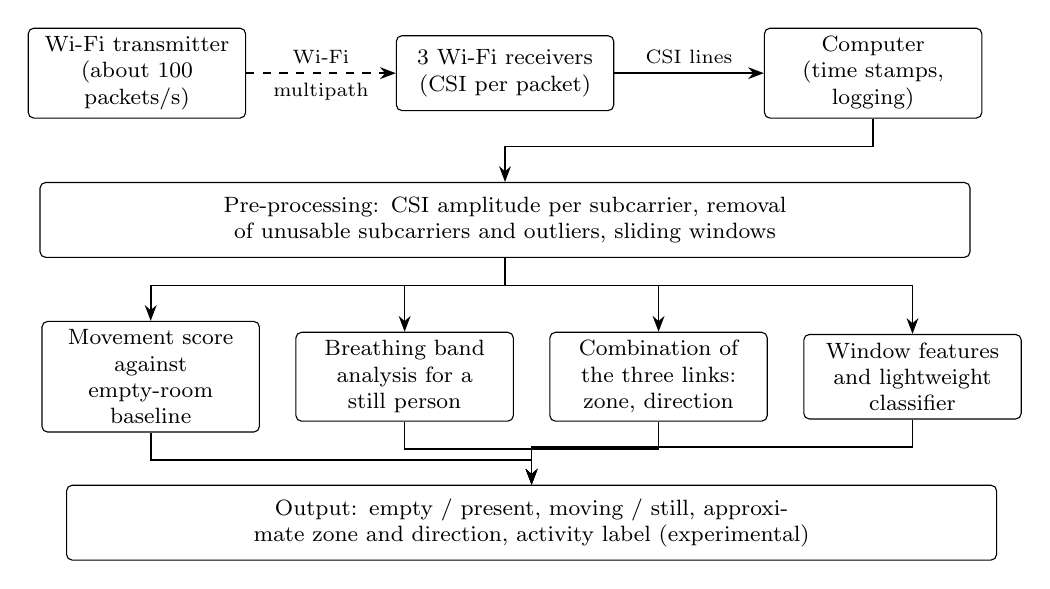
\begin{tikzpicture}[
  node distance=0.55cm and 0.7cm,
  box/.style={draw, rounded corners=2pt, align=center, font=\footnotesize, minimum height=0.95cm, text width=2.55cm, inner sep=3pt},
  wide/.style={box, text width=11.6cm},
  arr/.style={-{Stealth[length=2mm]}, semithick}]
  \node[box] (tx) {Wi-Fi transmitter\\(about 100 packets/s)};
  \node[box, right=1.9cm of tx] (rx) {3 Wi-Fi receivers\\(CSI per packet)};
  \node[box, right=1.9cm of rx] (pc) {Computer\\(time stamps, logging)};
  \draw[arr, dashed] (tx) -- node[above, font=\scriptsize]{Wi-Fi} node[below, font=\scriptsize]{multipath} (rx);
  \draw[arr] (rx) -- node[above, font=\scriptsize]{CSI lines} (pc);

  \node[wide, below=0.9cm of rx] (pre) {Pre-processing: CSI amplitude per subcarrier, removal of unusable subcarriers and outliers, sliding windows};
  \draw[arr] (pc.south) |- ([yshift=0.45cm]pre.north) -- (pre.north);

  \node[box, below=0.8cm of pre, xshift=-4.5cm] (mov) {Movement score\\against empty-room\\baseline};
  \node[box, right=0.45cm of mov] (br) {Breathing band\\analysis for a\\still person};
  \node[box, right=0.45cm of br] (loc) {Combination of\\the three links:\\zone, direction};
  \node[box, right=0.45cm of loc] (ml) {Window features\\and lightweight\\classifier};
  \foreach \n in {mov,br,loc,ml} \draw[arr] (pre.south) -- ++(0,-0.35) -| (\n.north);

  \node[wide, below=0.8cm of $(br.south)!0.5!(loc.south)$] (out) {Output: empty / present, moving / still, approximate zone and direction, activity label (experimental)};
  \foreach \n in {mov,br,loc,ml} \draw[arr] (\n.south) -- ++(0,-0.35) -| (out.north);
\end{tikzpicture}
\caption{Overview of the proposed sensing pipeline}
\label{fig:overview}
\end{figure}

On the computer, the processing is done in four stages.
\begin{enumerate}
  \item \textbf{Pre-processing.} The real and imaginary values of each subcarrier are converted to amplitude. Subcarriers that carry no signal are removed, outliers are filtered, and the stream is cut into short overlapping windows. Phase is not used as a main feature, because the raw phase reported by a commodity receiver contains random offsets, and cancelling them needs a second synchronised antenna that cannot be assumed on ordinary devices.
  \item \textbf{Presence and movement detection.} For each link, a movement score is computed from how strongly the amplitudes change inside a window. The score is compared with a threshold that is learned from a short recording of the empty room. This follows the basic observation, used since FIMD \cite{fimd}, that CSI is stable in a static room and bursts when something moves. For a person who is not walking, the system looks for a slow periodic component in the frequency range of human breathing, following the idea of DeMan \cite{deman}.
  \item \textbf{Coarse location and direction.} Each link runs its own detector. The position of movement is estimated from which links are disturbed and how strongly, and the direction is estimated from how this estimate changes over a few seconds. The result is a zone in the room, not an exact coordinate, and it is presented as such.
  \item \textbf{Learned recognition.} Features are extracted from every window, such as the energy of the change, its distribution over several speed bands and its distribution over groups of subcarriers. A lightweight classifier is trained on labelled recordings to separate a small set of activities and zones.
\end{enumerate}

Every learned model is evaluated by holding out complete recording sessions. Windows that are close in time overlap almost completely, so a random split of windows would place nearly identical samples in the training and the test set and would report accuracy that is too high. Holding out whole sessions avoids this.

\chapter{Literature Review}
This chapter reviews nineteen works on sensing people with commodity Wi-Fi. Section~\ref{sec:related} describes the existing systems, grouped by what they detect. Section~\ref{sec:comparison} compares them side by side. Section~\ref{sec:gap} discusses the limitations that remain, and Section~\ref{sec:contribution} states what this research proposes to add.

\section{Existing Systems / Related Works}
\label{sec:related}

\subsection{Motion and Presence Detection}
Xiao et al. \cite{fimd} proposed FIMD, one of the first motion detection systems built on CSI. The authors start from the weakness of RSS: it varies strongly by itself, so a slow movement is easily hidden and missed. Their key observation is that CSI stays stable over time in a static environment and shows burst patterns when motion takes place. FIMD extracts a feature from CSI that uses this temporal stability together with the diversity across subcarriers, and then treats motion detection as the search for outliers among normal feature values with the density-based clustering algorithm DBSCAN. A false alert filter and data fusion are added to improve accuracy. The system was implemented with commercial IEEE 802.11n network cards and tested in two indoor scenarios, where the CSI feature gave better detection and better resistance to narrowband interference than RSS. The paper established the principle that most later work builds on, but it only answers whether something moves, and a person who stands still is not covered.

Qian et al. \cite{pads} addressed a weakness of such detectors: they may fail when a person moves very slowly. Their system PADS extracts both the amplitude and the phase of CSI and shapes them into metrics that are sensitive to movement. It also uses the several antennas of a MIMO receiver, an aspect that the authors note had been studied much less than the diversity across subcarriers. The prototype on commercial Wi-Fi devices reports that human movement at various walking speeds is detected in about 97\% of cases on average. The limitation is that PADS relies on phase information and on several antennas; the paper itself notes that using a ``bad'' antenna by mistake can cause many false alarms.

Wu et al. \cite{deman} extended detection from moving people to stationary people with DeMan. Earlier approaches to stationary people needed a calibration of the channel profile in the empty environment for each scenario. DeMan uses the amplitude and phase of CSI to detect moving targets and, when there is no large movement, treats human breathing as the sign that a person is present. It searches the signal for the periodic pattern caused by the small motion of the chest. The authors report true positive rates of 94.82\% for moving and 93.33\% for stationary people and a true negative rate of 96.25\% for empty scenes, about 30\% better than previous approaches, with only a small number of earlier measurements needed to set the model parameters. The breathing pattern is fragile, however: the authors state that it can be destroyed by significant body motion or hidden by environmental noise.

\subsection{Through-the-Wall Detection}
Detecting people behind a wall is harder because the wall weakens the signal strongly. Zeng et al. \cite{thude} proposed T-HuDe for through-the-wall detection of an active person with commodity devices. The system first selects a suitable antenna, because the antennas perform differently, and applies a band-pass filter to remove noise. It then estimates the power spectrum over Doppler velocity with a Doppler-MUSIC method and uses statistics of this spectrum over time to decide whether a moving person is present. In two indoor environments, the true positive and true negative rates were above 93\% in most areas. The method is aimed at moving people and depends on choosing a good antenna.

Li et al. \cite{wiborder} looked at the opposite side of the same effect in WiBorder. Because Wi-Fi passes through walls, a sensing system often reacts to people outside the area of interest, which causes false alarms in applications such as intrusion detection. WiBorder is presented by its authors as the first method to determine a precise sensing boundary. It multiplies the CSI of one receiving antenna with the conjugate of the CSI of a second antenna. This removes the random phase offset that changes from packet to packet and at the same time amplifies the attenuation caused by the wall. From the result the authors build a metric that separates movement inside the room from movement behind the wall. Two case studies are reported: an intrusion detection system with a 99.4\% detection rate and a 0.68\% false alarm rate, and an area detection system with 97.03\% accuracy. The whole approach rests on having two antennas that share one oscillator.

Shen et al. \cite{alpd} used deep learning for through-the-wall presence detection in a system called ALPD. An attention mechanism selects the informative subcarriers automatically, and a bidirectional LSTM network captures how the CSI develops over time. An additional static feature improves detection when the person does not move. The data were collected with pairs of ordinary TP-Link routers, and the authors report average accuracy of up to about 96\%, with better behaviour than the benchmark methods when interference is present. They also show that using data from both directions of transmission makes training more stable. The price is the need for labelled training data and a model that is much heavier than a threshold.

Gu et al. \cite{wifileaks} studied the same capability as an attack. In WiFiLeaks, an attacker outside a room uses a commodity smartphone to listen passively to the signals of the Wi-Fi devices inside, without controlling the transmitter and without special radio equipment. The difficulty is that these signals are not sent at a regular, high rate. The authors combine outlier handling and wavelet denoising to strengthen the low-frequency information related to human presence, and they use the correlation among subcarriers as the feature, because a stationary person increases this correlation. With nine different transmitters and one smartphone in four settings, WiFiLeaks reached 83.33\% accuracy for presence and 100\% for absence at 20 metres between the monitoring device and the transmitter in through-the-wall scenarios. The work is important for this research in two ways: it shows that stationary presence can be sensed with modest hardware, and it shows that such sensing has a privacy cost that must be discussed.

\subsection{Activity Recognition}
Wang et al. \cite{eeyes} presented E-eyes, an early and influential system for recognising activities at home with existing Wi-Fi access points and devices. E-eyes separates in-place activities, such as cooking or brushing teeth, from walking movements, and identifies them by comparing the measured CSI with stored signal profiles. The idea behind it is that many home activities happen at one or a few fixed places, so a small number of profiles per place is sufficient. Profiles can be built in a semi-supervised way and updated to follow day-to-day changes. In two apartments, the system reached an average true positive rate above 96\% with a false positive rate below 1\% using a single access point. As a profile-matching method, it depends on profiles that were recorded in the same home and must be kept up to date.

Wang et al. \cite{carm} argued that such systems lacked a model that links changes in CSI to human activity in a quantitative way. Their system CARM rests on two models. The CSI-speed model relates the dynamics of the CSI values to the speed of human movement, and the CSI-activity model relates the movement speeds of different body parts to a specific activity. On the signal processing side, CARM removes noise with Principal Component Analysis (PCA), extracts features with the Discrete Wavelet Transform (DWT), and recognises activities with Hidden Markov Models. The authors report an average accuracy above 96\%. The journal version of the work \cite{carmjsac} adds further experiments and reports 96\% recognition accuracy together with robustness to environmental changes. CARM matters to the present research because it explains why detection works at all: the frequency of the change in CSI is tied to how fast the reflecting body part moves.

\subsection{Fall Detection}
Han et al. \cite{wifall} proposed WiFall, the first fall detector based on CSI and the baseline that later fall detectors are measured against. WiFall first finds abnormal sections in the CSI series with an anomaly detection algorithm and then separates falls from other activities with a one-class Support Vector Machine. Implemented on laptops with commercial 802.11n network cards, it reached 87\% detection precision with an 18\% false alarm rate on average. The false alarm rate shows the central difficulty of fall detection: activities such as sitting down quickly look similar to a fall.

Zhang et al. \cite{antifall} addressed this in Anti-Fall. The authors identify the difference of the CSI phase between two antennas as the feature that reliably segments falls and fall-like activities, and then use both phase and amplitude to separate real falls from the fall-like ones. In two indoor scenarios, Anti-Fall achieved a 10\% higher detection rate and a 10\% lower false alarm rate than WiFall on average. The same group later presented RT-Fall \cite{rtfall}, which segments and detects falls automatically in real time. It again uses the phase difference over two antennas, which the authors find to be a more sensitive base signal than amplitude, and it exploits a sharp decline of the power profile in the time-frequency domain that is characteristic of a fall. In four indoor scenarios, RT-Fall outperformed WiFall with 14\% higher sensitivity and 10\% higher specificity on average.

Palipana et al. \cite{falldefi} focused on the dependence on the environment. Their system FallDeFi analyses CSI in the time-frequency domain, uses a pre-screener to find fall-like events, and selects features that are resilient to changes in the environment. A pre-trained system reaches above 93\% average accuracy. When the environment changes, or when the system is trained in a different environment, the average accuracy is close to 80\%. The authors report that this is still clearly better than RT-Fall and CARM under the same conditions. The result is valuable because it states openly how much accuracy is lost outside the training environment.

Nguyen and Nguyen \cite{adafall} tried to improve this generalisation with adversarial data augmentation on the FallDeFi dataset. Their conclusion is modest: deep learning systems improved slightly in unseen domains, but the improvement was not significant. This is a useful negative result. It shows that robustness to new environments is not solved by a training technique alone.

\subsection{Vital Signs and Learning-Based Sensing}
Liu et al. \cite{vitalsigns} showed that the very small movements caused by breathing and heartbeat can be tracked during sleep with one access point and a single Wi-Fi device. Their system works on CSI in both the time and the frequency domain, estimates the breathing rate of one person and of two people in the same bed, and was tested in a laboratory and two apartments over three months. The authors report accuracy comparable to, or better than, approaches with dedicated sensors. The setting is favourable, since a sleeping person lies still between the two devices at a short distance, but the work proves that breathing is visible in commodity CSI, which is the basis for detecting a stationary person.

Yang et al. \cite{sensefi} built SenseFi, a library and benchmark for deep learning in Wi-Fi sensing. It compares multilayer perceptrons, convolutional networks, recurrent networks and their variants, transformers and combined CNN-RNN models on four datasets, two of them public and two collected by the authors, in terms of accuracy, model size, computational cost and transferability. One observation is directly relevant here: a shallow five-layer CNN gave good results on all datasets, while a deep ResNet-18 failed to generalise on one of them. A larger model is therefore not automatically better when the data are limited.

The same group proposed AutoFi \cite{autofi} to reduce the need for labelled data. Learning-based models suffer strongly from environmental dependency, and collecting well segmented and balanced samples in every new environment is not practical. AutoFi learns from unlabelled CSI samples that are captured at random, using a geometric self-supervised learning algorithm, and then transfers this knowledge to tasks defined by the user, such as gait recognition, activity recognition and gesture recognition. It was implemented on a pair of Atheros access points.

\subsection{Surveys}
Wang et al. \cite{survey2019} surveyed more than one hundred CSI-based behaviour recognition applications from the preceding six years. The survey describes the general structure of such systems as a sequence of base signal selection, signal pre-processing and identification, and it classifies the applications into pattern-based, model-based and deep learning-based approaches. It also lists the hardware used by these applications, which is dominated by the Intel 5300 network card and several Atheros chipsets, and it closes with the open issues of the field. The survey confirms the picture that emerges from the individual papers reviewed above.

\section{Comparative Analysis}
\label{sec:comparison}
Table~\ref{tab:comparison} places the reviewed systems side by side. The results in the last column are the figures reported by the authors of each work. They were obtained with different hardware, rooms, participants and metrics, so they show what each system claims and cannot be ranked against each other directly.

{\small
\setlength{\tabcolsep}{4pt}
\begin{longtable}{L{2.25cm}L{2.2cm}L{2.5cm}L{3.3cm}L{3.5cm}}
\caption{Comparison of the reviewed Wi-Fi sensing systems}\label{tab:comparison}\\
\toprule
\textbf{Work} & \textbf{Task} & \textbf{Hardware} & \textbf{Main technique} & \textbf{Reported result}\\
\midrule
\endfirsthead
\multicolumn{5}{l}{\small Table \thetable\ (continued)}\\
\toprule
\textbf{Work} & \textbf{Task} & \textbf{Hardware} & \textbf{Main technique} & \textbf{Reported result}\\
\midrule
\endhead
\bottomrule
\endfoot
FIMD \cite{fimd}, 2012 & Motion detection & Intel 5300 NIC & CSI stability feature, DBSCAN outlier detection & Better detection and interference resistance than RSS\\\addlinespace
PADS \cite{pads}, 2014 & Motion detection at varying speed & Intel 5300 NIC, several antennas & Amplitude and phase metrics, antenna diversity & About 97\% of movements detected\\\addlinespace
DeMan \cite{deman}, 2015 & Moving and stationary presence & Intel 5300 NIC & Amplitude and phase for motion, breathing pattern for still person & 94.82\% (moving), 93.33\% (still), 96.25\% (empty)\\\addlinespace
T-HuDe \cite{thude}, 2019 & Through-wall detection of active person & Intel 5300 NIC & Antenna selection, Doppler-MUSIC spectrum statistics & Above 93\% true positive and true negative in most areas\\\addlinespace
WiBorder \cite{wiborder}, 2020 & Sensing boundary, intrusion & Intel 5300 NIC, two RX antennas & Conjugate multiplication between antennas & 99.4\% detection, 0.68\% false alarm\\\addlinespace
ALPD \cite{alpd}, 2023 & Through-wall presence & TP-Link routers & Attention over subcarriers, bidirectional LSTM & Up to about 96\% accuracy\\\addlinespace
WiFiLeaks \cite{wifileaks}, 2024 & Through-wall stationary presence (attack) & Commodity smartphone, passive & Wavelet denoising, subcarrier correlation & 83.33\% presence, 100\% absence at 20 m\\\addlinespace
E-eyes \cite{eeyes}, 2014 & Activity identification & Intel 5300 NIC, one AP & Matching against CSI profiles & Over 96\% true positive, under 1\% false positive\\\addlinespace
CARM \cite{carm,carmjsac}, 2015/2017 & Activity recognition & Intel 5300 NIC & CSI-speed and CSI-activity models, PCA, DWT, HMM & About 96\% accuracy\\\addlinespace
WiFall \cite{wifall}, 2014 & Fall detection & Intel 5300 NIC & Anomaly detection, one-class SVM & 87\% precision, 18\% false alarm\\\addlinespace
Anti-Fall \cite{antifall}, 2015 & Fall detection & Intel 5300 NIC, two antennas & Phase difference for segmentation, phase and amplitude features & 10\% higher detection, 10\% lower false alarm than WiFall\\\addlinespace
RT-Fall \cite{rtfall}, 2017 & Real-time fall detection & Intel 5300 NIC, two antennas & Phase difference, power decline pattern & 14\% higher sensitivity, 10\% higher specificity than WiFall\\\addlinespace
FallDeFi \cite{falldefi}, 2018 & Fall detection across environments & Intel 5300 NIC & Time-frequency features, feature selection & Above 93\% pre-trained, close to 80\% in changed environment\\\addlinespace
Nguyen and Nguyen \cite{adafall}, 2020 & Fall detection in unseen environments & FallDeFi dataset & Adversarial data augmentation & Slight, not significant improvement\\\addlinespace
Liu et al. \cite{vitalsigns}, 2015 & Breathing and heart rate in sleep & Laptop NIC and one AP & Time and frequency analysis of CSI & Comparable to dedicated sensors\\\addlinespace
AutoFi \cite{autofi}, 2022 & Gait, activity, gesture with few labels & Atheros APs, public datasets & Geometric self-supervised learning & Cross-task transfer from unlabelled data\\\addlinespace
SenseFi \cite{sensefi}, 2023 & Benchmark of deep models & Four datasets & MLP, CNN, RNN variants, transformer & Shallow CNN good on all datasets\\
\end{longtable}
}

Several patterns can be read from the comparison.

\textbf{From hand-made features to learned models.} The early systems rely on signal processing and simple decision rules: an outlier test in FIMD, statistical metrics in PADS, a breathing model in DeMan and profile matching in E-eyes. The middle period adds classical machine learning, such as the one-class SVM in WiFall and the Hidden Markov Models in CARM. The recent systems, ALPD, AutoFi and the models benchmarked in SenseFi, learn the features themselves. The learned systems report high accuracy, but they need labelled data, and the works that test them outside their training environment report clear losses \cite{falldefi,adafall}.

\textbf{From amplitude to phase and several antennas.} FIMD and WiFall work mainly with amplitude. Later systems obtain their gains from phase: PADS and DeMan add phase information, Anti-Fall and RT-Fall build on the phase difference between two antennas, and WiBorder multiplies the CSI of two antennas. The improvement from WiFall to RT-Fall comes to a large part from this change of the base signal.

\textbf{The same few hardware platforms.} Thirteen of the seventeen entries in Table~\ref{tab:comparison} used the Intel 5300 network card or data recorded with it, and two of the four SenseFi datasets were recorded with it as well. The remaining works used routers or a smartphone.

\textbf{Moving people are detected much more reliably than still people.} Only DeMan, WiFiLeaks, ALPD and the vital sign system of Liu et al. deal with a person who does not move, and each of them needs special care for this case: a breathing model, a correlation feature or an additional static feature.

\textbf{One task per system.} Each system solves one task. A direct comparison across tasks, on the same hardware and the same data, is only available for deep learning models through SenseFi, and only for activity and gesture recognition.

\section{Research Gap / Existing Limitations}
\label{sec:gap}
The review shows that sensing people with Wi-Fi is well established, but it also shows limitations that the present research can address.

\textbf{Dependence on multi-antenna hardware.} The techniques behind the best results need at least two receiving antennas on a shared oscillator \cite{antifall,rtfall,wiborder}, a choice among several antennas \cite{thude} or the full antenna array of a MIMO receiver \cite{pads}. Most of them were built on one specific network card, the Intel 5300. It is therefore unclear how much of the reported performance can be reached with ordinary commodity Wi-Fi devices, on which the cleaned phase signal that these methods use cannot be assumed to be available.

\textbf{Dependence on the environment.} Profile-based and learning-based systems are tied to the room in which they were set up. E-eyes must update its profiles to follow daily changes \cite{eeyes}. FallDeFi loses more than ten percentage points when the environment changes \cite{falldefi}, adversarial augmentation helps only slightly \cite{adafall}, and AutoFi was motivated by exactly this problem \cite{autofi}. Many of the high accuracies in Table~\ref{tab:comparison} were measured in the environment of training, and only a few works report what happens outside it.

\textbf{Stationary people.} A still person is detected through breathing \cite{deman,vitalsigns} or through subtle changes in subcarrier correlation \cite{wifileaks}. These signals are small, are easily covered by noise or by the movement of other people, and were demonstrated in favourable conditions such as a sleeping person between two devices. Reliable detection of a still person with ordinary hardware remains open.

\textbf{No precise location from one link.} A single link can tell that something moves, but not where. Without a boundary method such as WiBorder, which again needs two antennas, a detector also reacts to movement outside the area of interest \cite{wiborder}. How far several cheap links can replace this is not answered by the reviewed works.

\textbf{Separate systems for separate tasks.} Presence, location, activity and breathing are treated by different systems with different hardware and evaluation methods. For someone who wants to build one installation, the literature does not say what a single low-cost set-up can achieve across these tasks.

\textbf{Privacy.} WiFiLeaks shows that presence can be inferred from outside a room without the knowledge of the people inside \cite{wifileaks}. Most sensing papers treat Wi-Fi sensing as privacy friendly because it does not record images, and they do not discuss this risk.

\section{Proposed Contribution}
\label{sec:contribution}
In response to these gaps, this research proposes the following contributions.

\begin{enumerate}
  \item \textbf{A sensing platform built only from commodity Wi-Fi devices.} The system uses four commodity Wi-Fi devices, one transmitter and three receivers, and needs no special radio equipment. The device settings, the data format and the recording tools will be documented so that the set-up can be repeated by others with the same widely available parts.
  \item \textbf{An amplitude-based detection pipeline suited to this hardware.} Because the phase-difference techniques of the literature cannot be relied on with ordinary devices, the pipeline is built on the amplitude of the subcarriers and compensates with several links. It detects presence and movement against a short empty-room baseline, in the spirit of FIMD \cite{fimd}, and looks for breathing to detect a still person, in the spirit of DeMan \cite{deman}.
  \item \textbf{Coarse location and direction from several links.} The three links are combined to estimate the zone in which movement happens and the direction in which it proceeds. The output is described as approximate, and its error will be measured against marked positions in the room.
  \item \textbf{An evaluation that does not overstate the result.} All learned models are tested on complete recording sessions that were not used for training, and the experiments are repeated after changing the layout of the room and the placement of the devices. The research will report where the system fails, for example for a still person or for movement outside the links, in the same detail as where it succeeds.
  \item \textbf{A comparison of simple and learned methods on the same data.} Threshold-based detection, a lightweight classifier and, if the amount of data allows it, a small neural network of the kind recommended by SenseFi \cite{sensefi} will be compared on identical recordings. This shows whether the added complexity is justified on this hardware.
  \item \textbf{An account of the privacy implications.} The research will discuss what the measured capability means for the privacy of people near ordinary Wi-Fi devices, with reference to WiFiLeaks \cite{wifileaks}, and all recordings of people will be made only with their consent.
\end{enumerate}

The expected outcome is a clear, measured answer to the question of how far presence, movement and coarse location can be sensed with resources that are cheap and widely available, together with an open description of the limits.

\chapter{Preliminary Design and Planning}
This chapter turns the proposal of the first two chapters into a first design. It lists what the system must do and how well it must do it, shows how a user works with it and how the data flows at run time, describes the preliminary architecture and the tools, and closes with the project timeline and the risks. The design is preliminary. It records the decisions taken so far and will be refined when the systematic recordings begin.

\section{Functional Requirements}
The functional requirements follow from the objectives in Chapter~1. Each requirement names the objective it serves, so that later chapters can report against it. Table~\ref{tab:fr} lists them.

{\small
\setlength{\tabcolsep}{4pt}
\begin{longtable}{L{1.1cm}L{10.6cm}L{1.9cm}}
\caption{Functional requirements}\label{tab:fr}\\
\toprule
\textbf{ID} & \textbf{Requirement} & \textbf{Objective}\\
\midrule
\endfirsthead
\multicolumn{3}{l}{\small Table \thetable\ (continued)}\\
\toprule
\textbf{ID} & \textbf{Requirement} & \textbf{Objective}\\
\midrule
\endhead
\bottomrule
\endfoot
FR1 & The transmitter shall send packets at a fixed, configurable rate. & 2\\\addlinespace
FR2 & Each receiver shall read the CSI of every packet it receives from the transmitter and forward it to the computer. & 2\\\addlinespace
FR3 & The computer shall read the three receiver streams at the same time, add a time stamp and the identity of the link to every packet, and store the raw data of a session in a file. & 2\\\addlinespace
FR4 & The operator shall be able to start and stop a recording session and to attach a label to it: the activity, the zone, the participant code and the room layout. & 2, 6\\\addlinespace
FR5 & The system shall learn an empty-room baseline for every link from a short calibration recording. & 3\\\addlinespace
FR6 & The system shall decide for every time window whether the room is empty or occupied by a moving person. & 3\\\addlinespace
FR7 & When no movement is found, the system shall search the signal for a breathing pattern and report a person who is present but still. & 4\\\addlinespace
FR8 & The system shall combine the three links into an approximate zone of the movement and a direction of movement. & 5\\\addlinespace
FR9 & The system shall extract features from every window and train a lightweight classifier on the labelled sessions. & 6\\\addlinespace
FR10 & The system shall evaluate every learned model on complete sessions that were not used for training and report accuracy together with the confusion between classes. & 7\\\addlinespace
FR11 & The system shall show the current state on a live display: empty or present, moving or still, zone and direction. & 3 to 5\\\addlinespace
FR12 & The system shall export the results of an evaluation so that they can be repeated and included in the report. & 7\\
\end{longtable}
}

\section{Non-Functional Requirements}
The non-functional requirements describe the qualities that the system must have besides its functions. Several of them come directly from the research gap in Section~\ref{sec:gap}: the hardware must stay cheap, the results must be honest, and the privacy of the people in the room must be respected. Where a number is given it is a target for the design. The values that are finally reached will be measured and reported.

{\small
\setlength{\tabcolsep}{4pt}
\begin{longtable}{L{1.3cm}L{2.7cm}L{9.6cm}}
\caption{Non-functional requirements}\label{tab:nfr}\\
\toprule
\textbf{ID} & \textbf{Quality} & \textbf{Requirement}\\
\midrule
\endfirsthead
\multicolumn{3}{l}{\small Table \thetable\ (continued)}\\
\toprule
\textbf{ID} & \textbf{Quality} & \textbf{Requirement}\\
\midrule
\endhead
\bottomrule
\endfoot
NFR1 & Low cost & The sensing hardware consists only of commodity Wi-Fi devices. No special radio equipment is needed.\\\addlinespace
NFR2 & Packet rate & Every link should deliver CSI at a steady rate close to the transmission rate of about 100 packets per second.\\\addlinespace
NFR3 & Responsiveness & The live display should follow a change in the room within a few seconds. The exact delay depends on the window length and will be measured.\\\addlinespace
NFR4 & Honest evaluation & No window of a test session may appear in the training data. Results are reported per session and also after a change of the room layout or of the device placement.\\\addlinespace
NFR5 & Robustness & A lost packet, a burst of interference or a receiver that is unplugged must not stop the recording. Windows with too few packets are marked and left out of the decision.\\\addlinespace
NFR6 & Short set-up & Installing the system in a new room should need only the placement of the devices and a short recording of the empty room.\\\addlinespace
NFR7 & Reproducibility & The device settings, the data format, the placement of the devices and the processing parameters are documented so that the set-up can be repeated by others.\\\addlinespace
NFR8 & Privacy & Recordings of people are made only with their consent. The stored data contain CSI values and labels, and no names, images or sound.\\\addlinespace
NFR9 & Lightweight processing & The detection and the classifier must run in real time on an ordinary laptop without a graphics card.\\\addlinespace
NFR10 & Maintainability & Acquisition, pre-processing, detection, fusion and evaluation are separate modules, so that one method can be replaced without changing the others.\\
\end{longtable}
}

\section{Use Case Diagram}
Figure~\ref{fig:usecase} shows the use cases of the system. There are two actors. The \emph{operator} is the researcher who installs the devices, calibrates the system, records and labels sessions, and trains and evaluates the models. The \emph{observer} is the person who only wants to know the state of the room, for example a caregiver or the owner of the room. The person who is sensed does not appear as an actor. This is intended: the sensing is device-free, so the occupant does not carry anything and does not interact with the system. The occupant is involved only before a recording, when consent is asked.

\begin{figure}[htbp]
\centering\setstretch{1}
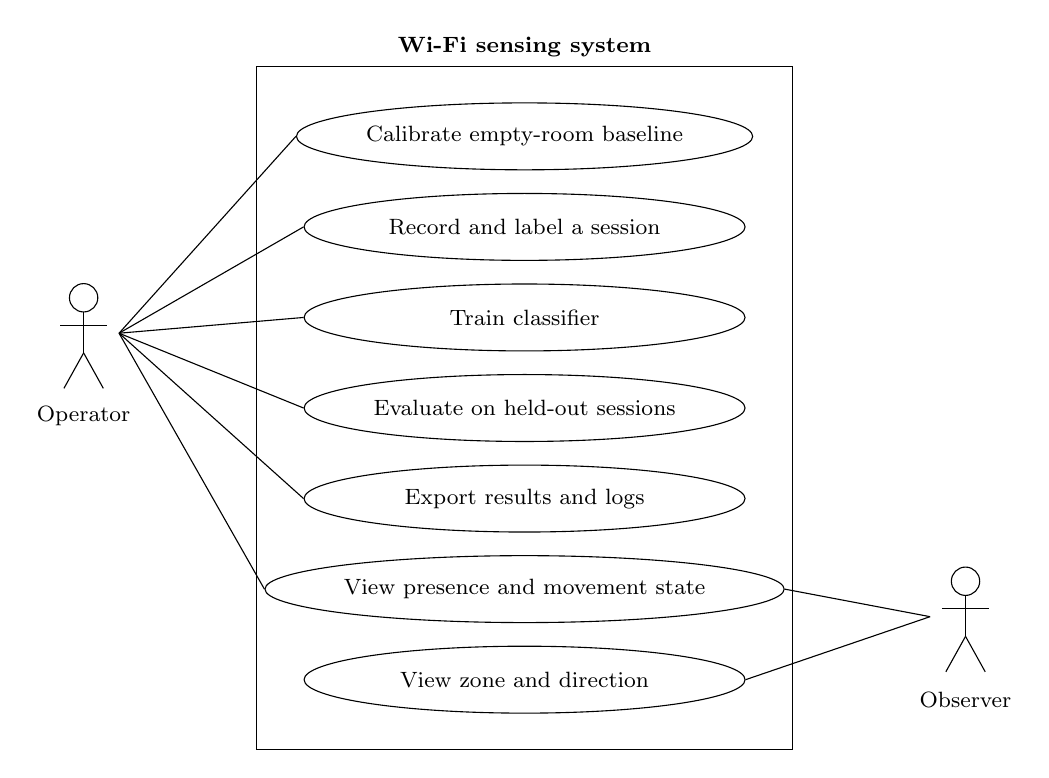
\begin{tikzpicture}[
  uc/.style={draw, ellipse, align=center, font=\footnotesize, minimum width=5.6cm, minimum height=0.85cm, inner sep=1pt}]
  \node[uc] (u1) at (0,0) {Calibrate empty-room baseline};
  \node[uc] (u2) at (0,-1.15) {Record and label a session};
  \node[uc] (u3) at (0,-2.3) {Train classifier};
  \node[uc] (u4) at (0,-3.45) {Evaluate on held-out sessions};
  \node[uc] (u5) at (0,-4.6) {Export results and logs};
  \node[uc] (u6) at (0,-5.75) {View presence and movement state};
  \node[uc] (u7) at (0,-6.9) {View zone and direction};
  \node[draw, fit=(u1)(u7), inner xsep=0.5cm, inner ysep=0.45cm,
        label={[font=\footnotesize\bfseries]above:Wi-Fi sensing system}] (sys) {};
  \actor{op}{-5.6,-2.6}{Operator}
  \actor{ob}{5.6,-6.2}{Observer}
  \foreach \u in {u1,u2,u3,u4,u5,u6} \draw (op-e) -- (\u.west);
  \foreach \u in {u6,u7} \draw (ob-w) -- (\u.east);
\end{tikzpicture}
\caption{Use case diagram of the proposed system}
\label{fig:usecase}
\end{figure}

The use cases are described briefly below.
\begin{description}[leftmargin=0.6cm,itemsep=2pt]
  \item[Calibrate empty-room baseline.] The operator makes sure that the room is empty and starts a short recording. The system stores the normal variation of every link and derives the detection threshold from it.
  \item[Record and label a session.] The operator enters the label of the session, starts the recording, and stops it when the activity is finished. The raw CSI of the three links is stored together with the label.
  \item[Train classifier.] The operator selects the sessions that are used for training. The system extracts the window features and trains the classifier.
  \item[Evaluate on held-out sessions.] The operator selects sessions that were not used for training. The system reports the accuracy and the confusion between the classes.
  \item[Export results and logs.] The operator saves the results and the settings of an evaluation.
  \item[View presence and movement state.] The operator or the observer reads from the live display whether the room is empty or occupied and whether the person moves or is still.
  \item[View zone and direction.] The observer reads the approximate zone and the direction of the movement.
\end{description}

\section{Activity Diagram}
Figure~\ref{fig:activity} shows the activity of the system while it is running. The same steps are repeated for every new window of data. Movement is tested first, because it gives the strongest signal. The search for breathing is used only when no movement is found, since body movement hides the much smaller breathing pattern, as noted for DeMan \cite{deman}.

\begin{figure}[htbp]
\centering\setstretch{1}
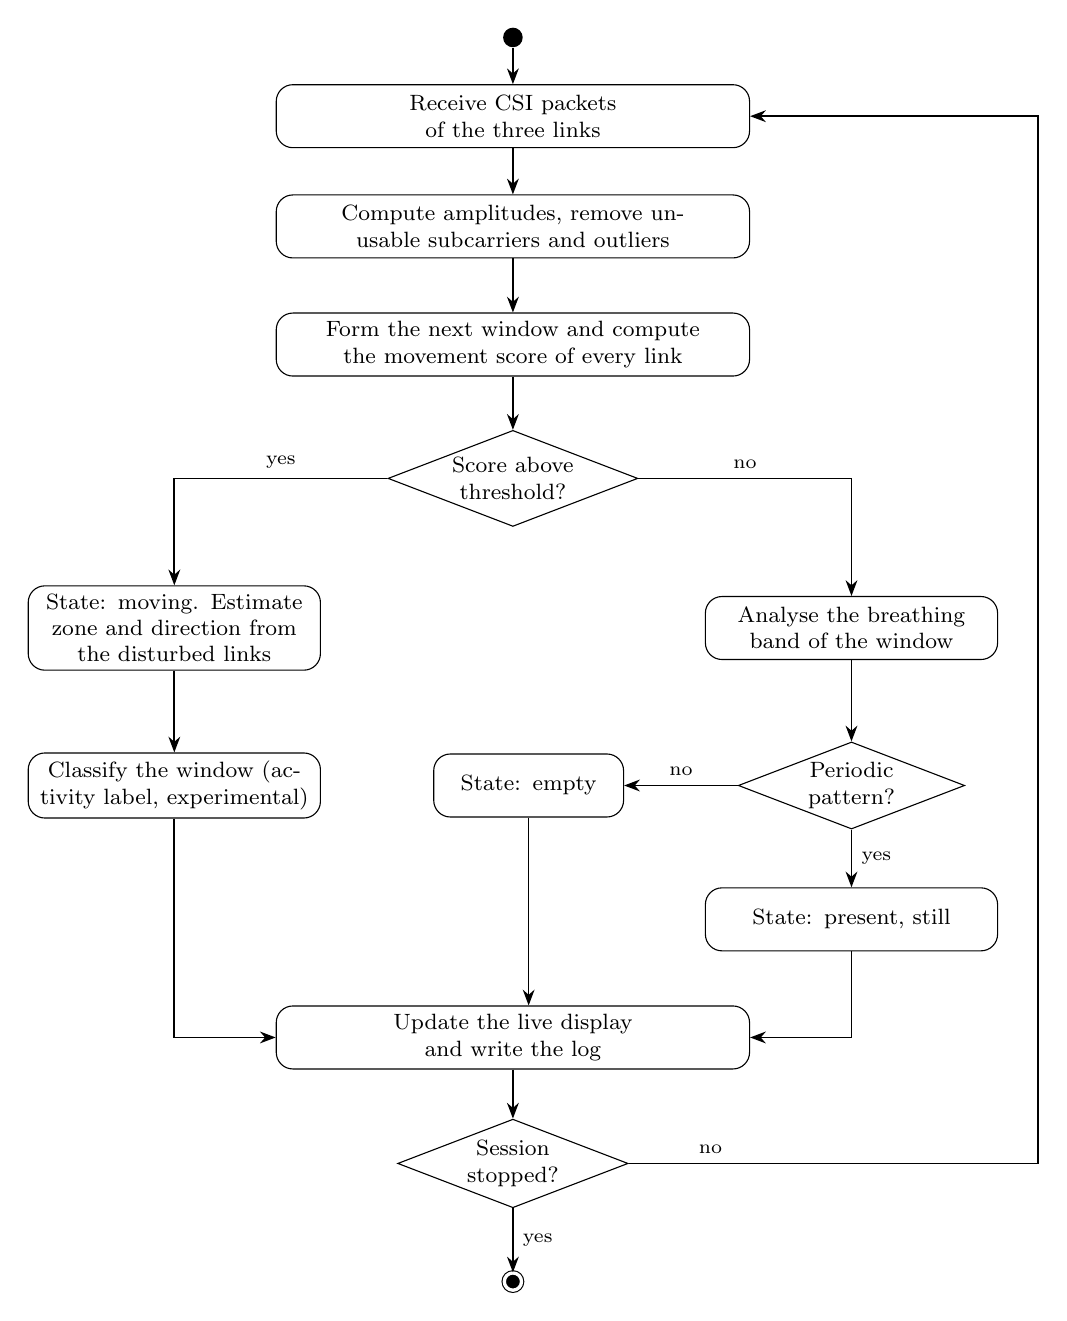
\begin{tikzpicture}[
  act/.style={draw, rounded corners=6pt, align=center, font=\footnotesize, minimum height=0.8cm, text width=5.8cm, inner sep=3pt},
  side/.style={act, text width=3.5cm},
  dec/.style={draw, diamond, aspect=2.6, align=center, font=\footnotesize, inner sep=1pt},
  arr/.style={-{Stealth[length=2mm]}, semithick},
  lab/.style={font=\scriptsize}]
  \node[circle, fill, inner sep=2.5pt] (start) at (0,0) {};
  \node[act] (cap) at (0,-1.0) {Receive CSI packets\\of the three links};
  \node[act] (pre) at (0,-2.4) {Compute amplitudes, remove unusable subcarriers and outliers};
  \node[act] (win) at (0,-3.9) {Form the next window and compute the movement score of every link};
  \node[dec] (d1) at (0,-5.6) {Score above\\threshold?};
  \node[side] (mov) at (-4.3,-7.5) {State: moving. Estimate zone and direction from the disturbed links};
  \node[side] (cls) at (-4.3,-9.5) {Classify the window (activity label, experimental)};
  \node[side] (br) at (4.3,-7.5) {Analyse the breathing band of the window};
  \node[dec] (d2) at (4.3,-9.5) {Periodic\\pattern?};
  \node[side] (still) at (4.3,-11.2) {State: present, still};
  \node[side, text width=2.2cm] (empty) at (0.2,-9.5) {State: empty};
  \node[act] (upd) at (0,-12.7) {Update the live display\\and write the log};
  \node[dec] (d3) at (0,-14.3) {Session\\stopped?};
  \node[circle, draw, double, double distance=1.2pt, fill, inner sep=2.2pt] (end) at (0,-15.8) {};

  \draw[arr] (start) -- (cap);
  \draw[arr] (cap) -- (pre);
  \draw[arr] (pre) -- (win);
  \draw[arr] (win) -- (d1);
  \draw[arr] (d1.west) -| node[lab, above, pos=0.25] {yes} (mov.north);
  \draw[arr] (d1.east) -| node[lab, above, pos=0.25] {no} (br.north);
  \draw[arr] (mov) -- (cls);
  \draw[arr] (br) -- (d2);
  \draw[arr] (d2.south) -- node[lab, right] {yes} (still.north);
  \draw[arr] (d2.west) -- node[lab, above] {no} (empty.east);
  \draw[arr] (cls.south) |- (upd.west);
  \draw[arr] (still.south) |- (upd.east);
  \draw[arr] (empty.south) -- (empty.south |- upd.north);
  \draw[arr] (upd) -- (d3);
  \draw[arr] (d3.south) -- node[lab, right] {yes} (end);
  \draw[arr] (d3.east) -- node[lab, above, pos=0.2] {no} ++(5.2,0) |- (cap.east);
\end{tikzpicture}
\caption{Activity diagram of the run-time processing}
\label{fig:activity}
\end{figure}

\section{Preliminary System Architecture}
Figure~\ref{fig:architecture} shows the preliminary architecture. It has four layers, and each layer only uses the layer directly below it. Figure~\ref{fig:overview} in Chapter~1 showed the flow of the data. The figure here shows the components and where they run.

\begin{figure}[htbp]
\centering\setstretch{1}
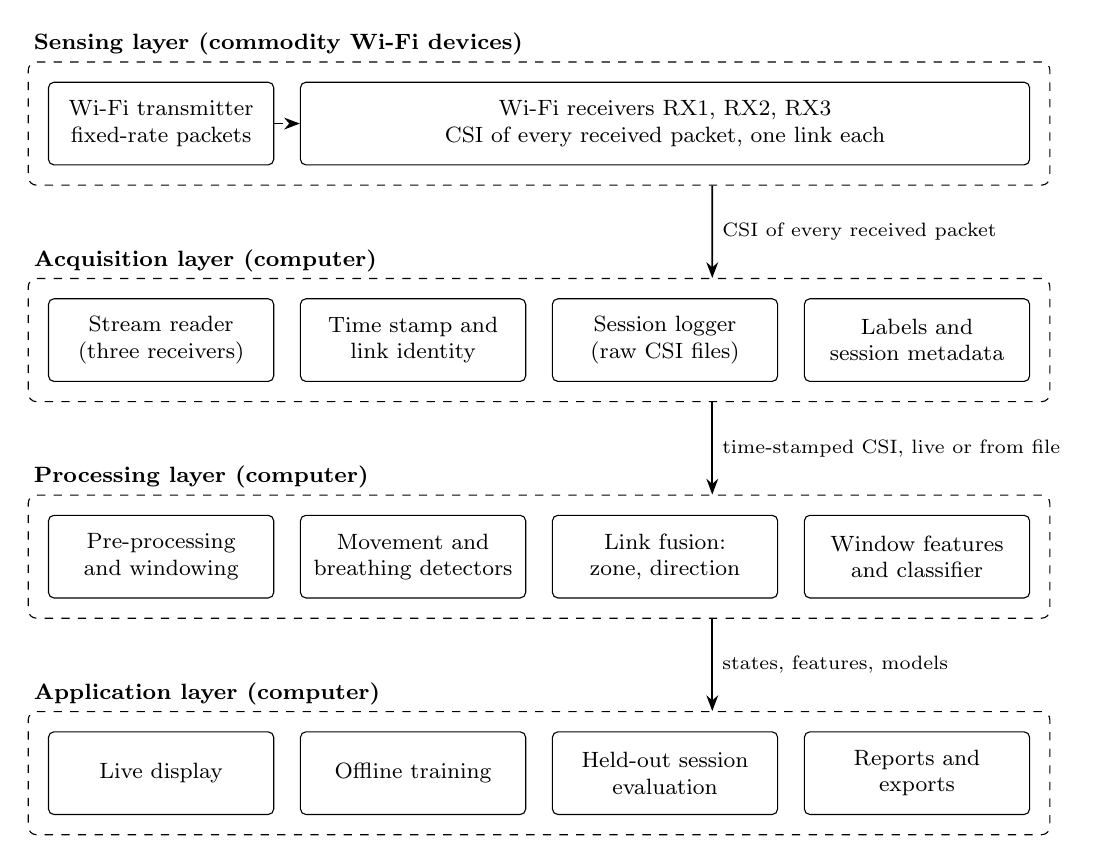
\begin{tikzpicture}[
  comp/.style={draw, rounded corners=2pt, align=center, font=\footnotesize, minimum height=1.05cm, text width=2.65cm, inner sep=3pt},
  layer/.style={draw, dashed, rounded corners=3pt, inner xsep=0.25cm, inner ysep=0.25cm},
  lname/.style={font=\footnotesize\bfseries, anchor=south west, inner sep=2pt},
  arr/.style={-{Stealth[length=2mm]}, semithick},
  lab/.style={font=\scriptsize, right}]
  % sensing layer
  \node[comp] (tx) at (-4.8,0) {Wi-Fi transmitter\\fixed-rate packets};
  \node[comp, text width=9.05cm] (rx) at (1.6,0) {Wi-Fi receivers RX1, RX2, RX3\\CSI of every received packet, one link each};
  \draw[arr, dashed] (tx) -- (rx);
  \node[layer, fit=(tx)(rx)] (l1) {};
  \node[lname] at (l1.north west) {Sensing layer (commodity Wi-Fi devices)};
  % acquisition layer
  \node[comp] (ser) at (-4.8,-2.75) {Stream reader\\(three receivers)};
  \node[comp] (ts) at (-1.6,-2.75) {Time stamp and\\link identity};
  \node[comp] (log) at (1.6,-2.75) {Session logger\\(raw CSI files)};
  \node[comp] (meta) at (4.8,-2.75) {Labels and\\session metadata};
  \node[layer, fit=(ser)(meta)] (l2) {};
  \node[lname] at (l2.north west) {Acquisition layer (computer)};
  % processing layer
  \node[comp] (pp) at (-4.8,-5.5) {Pre-processing\\and windowing};
  \node[comp] (det) at (-1.6,-5.5) {Movement and\\breathing detectors};
  \node[comp] (fus) at (1.6,-5.5) {Link fusion:\\zone, direction};
  \node[comp] (ml) at (4.8,-5.5) {Window features\\and classifier};
  \node[layer, fit=(pp)(ml)] (l3) {};
  \node[lname] at (l3.north west) {Processing layer (computer)};
  % application layer
  \node[comp] (ui) at (-4.8,-8.25) {Live display};
  \node[comp] (tr) at (-1.6,-8.25) {Offline training};
  \node[comp] (ev) at (1.6,-8.25) {Held-out session\\evaluation};
  \node[comp] (ex) at (4.8,-8.25) {Reports and\\exports};
  \node[layer, fit=(ui)(ex)] (l4) {};
  \node[lname] at (l4.north west) {Application layer (computer)};

  \draw[arr] ([xshift=2.2cm]l1.south) -- node[lab] {CSI of every received packet} ([xshift=2.2cm]l2.north);
  \draw[arr] ([xshift=2.2cm]l2.south) -- node[lab] {time-stamped CSI, live or from file} ([xshift=2.2cm]l3.north);
  \draw[arr] ([xshift=2.2cm]l3.south) -- node[lab] {states, features, models} ([xshift=2.2cm]l4.north);
\end{tikzpicture}
\caption{Preliminary layered architecture of the system}
\label{fig:architecture}
\end{figure}

\textbf{Sensing layer.} The transmitter and the three receivers are commodity Wi-Fi devices. The transmitter only sends packets. Each receiver forms one link with the transmitter, reads the CSI of every packet from its Wi-Fi driver and forwards it to the computer. The receivers do no processing, which keeps them simple and identical.

\textbf{Acquisition layer.} A reader on the computer listens to the three receivers at the same time. Every packet gets a time stamp and the identity of its link. The logger writes the raw data of a session to a file, and the label entered by the operator is stored with it. Raw data are always kept, so that every later result can be computed again from the original recordings.

\textbf{Processing layer.} The pre-processing converts the CSI to amplitudes, removes the subcarriers that carry no signal, filters outliers and forms the windows. The detectors compute the movement score and the breathing analysis for every link. The fusion component combines the three links into a zone and a direction. The last component extracts the window features and applies the classifier. The layer takes its input either from the live stream or from a stored session, so the same code is used for the live display and for the experiments.

\textbf{Application layer.} The live display shows the current state. Training and evaluation run offline on stored sessions. The evaluation component is responsible for the split by session, so that this rule is enforced in one place and cannot be bypassed by a single experiment.

\section{Technology Stack}
Table~\ref{tab:stack} lists the tools selected for the project. They were chosen because they are free, widely used and sufficient for the hardware. The tools on the computer may still change during the next stage, for example if a small neural network is added to the comparison.

% CONFIRM: adjust the tools below to what the group actually uses.
\begin{table}[htbp]
\centering
\small
\caption{Technology stack}\label{tab:stack}
\begin{tabular}{L{3.0cm}L{4.4cm}L{6.0cm}}
\toprule
\textbf{Part} & \textbf{Technology} & \textbf{Purpose}\\
\midrule
Sensing hardware & Four commodity Wi-Fi devices & One transmitter and three receivers\\\addlinespace
CSI extraction & CSI reporting of the Wi-Fi driver on the receivers & Fixed-rate transmission, reading CSI for every received packet\\\addlinespace
Acquisition & Python & Reading the three receiver streams in parallel, time stamps, session files\\\addlinespace
Signal processing & Python with NumPy and SciPy & Amplitude, outlier filtering, windows, frequency analysis of the breathing band\\\addlinespace
Machine learning & scikit-learn; PyTorch only if a small CNN is added & Lightweight classifiers, split by session, metrics\\\addlinespace
Visualisation & Matplotlib & Live display and figures for the report\\\addlinespace
Storage & Plain text or CSV files per session with a metadata file & Raw CSI, labels, room layout, device placement\\\addlinespace
Project tools & Git, \LaTeX & Version control of the code, writing of the reports\\
\bottomrule
\end{tabular}
\end{table}

\section{Project Timeline / Gantt Chart}
The work is planned over the three thesis stages P1, P2 and P3. Figure~\ref{fig:gantt} shows the plan, with every stage divided into four parts of equal length. P1 covers the study of the literature, the set-up of the hardware and the design of the processing pipeline. P2 is the main period of data collection and of the detection methods. P3 is used for the experiments after changes of the environment, for the comparison of the methods and for writing the thesis.

\begin{figure}[htbp]
\centering\setstretch{1}
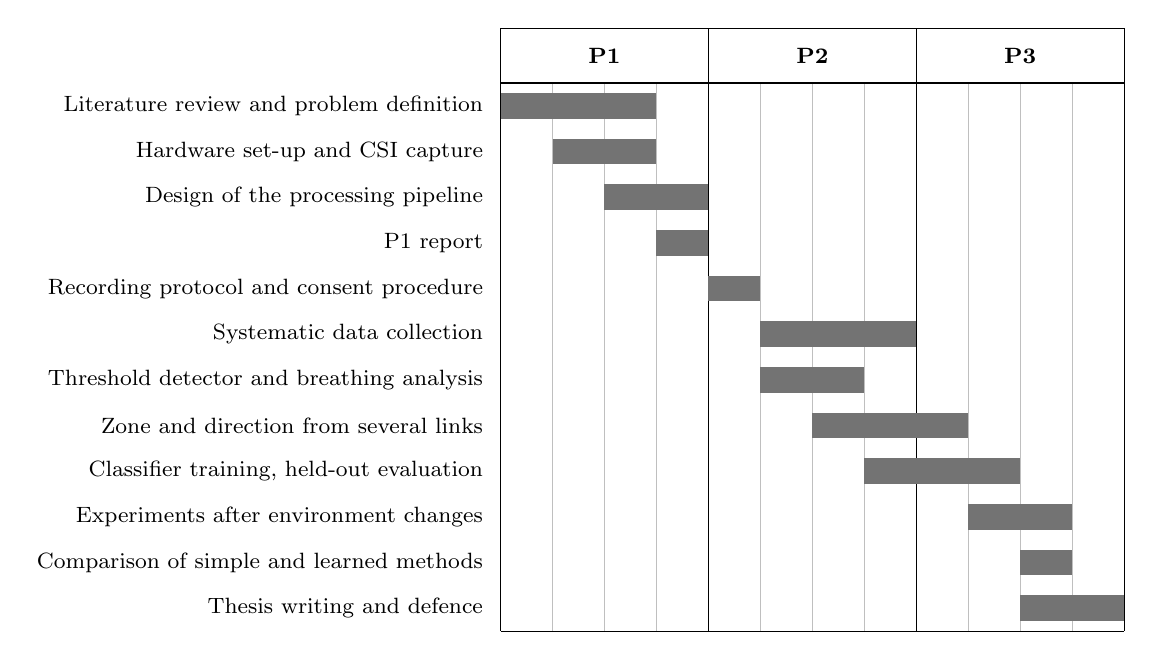
\begin{tikzpicture}[x=0.66cm, y=-0.58cm, font=\footnotesize]
  % header
  \foreach \s/\name in {0/P1, 4/P2, 8/P3} {
    \draw (\s,-1.2) rectangle (\s+4,0);
    \node at (\s+2,-0.6) {\textbf{\name}};
  }
  % grid
  \foreach \c in {0,...,12} \draw[black!25] (\c,0) -- (\c,12);
  \foreach \c in {0,4,8,12} \draw (\c,0) -- (\c,12);
  \draw (0,0) -- (12,0);
  \draw (0,12) -- (12,12);
  % tasks: row / start / end / name
  \foreach \row/\s/\e/\task in {
    0/0/3/{Literature review and problem definition},
    1/1/3/{Hardware set-up and CSI capture},
    2/2/4/{Design of the processing pipeline},
    3/3/4/{P1 report},
    4/4/5/{Recording protocol and consent procedure},
    5/5/8/{Systematic data collection},
    6/5/7/{Threshold detector and breathing analysis},
    7/6/9/{Zone and direction from several links},
    8/7/10/{Classifier training, held-out evaluation},
    9/9/11/{Experiments after environment changes},
    10/10/11/{Comparison of simple and learned methods},
    11/10/12/{Thesis writing and defence}} {
    \node[anchor=east] at (-0.15,\row+0.5) {\task};
    \fill[black!55] (\s,\row+0.22) rectangle (\e,\row+0.78);
  }
\end{tikzpicture}
\caption{Project timeline over the three thesis stages}
\label{fig:gantt}
\end{figure}

\section{Risk Management}
Table~\ref{tab:risk} lists the main risks of the project with their likelihood, their impact and the planned response. Most of them are technical and come from the limits of the hardware that were discussed in Section~\ref{sec:gap}.

{\small
\setlength{\tabcolsep}{4pt}
\begin{longtable}{L{3.4cm}L{2.1cm}L{1.5cm}L{6.4cm}}
\caption{Risks and planned responses}\label{tab:risk}\\
\toprule
\textbf{Risk} & \textbf{Likelihood} & \textbf{Impact} & \textbf{Planned response}\\
\midrule
\endfirsthead
\multicolumn{4}{l}{\small Table \thetable\ (continued)}\\
\toprule
\textbf{Risk} & \textbf{Likelihood} & \textbf{Impact} & \textbf{Planned response}\\
\midrule
\endhead
\bottomrule
\endfoot
A still person cannot be detected reliably from CSI amplitude alone & High & Medium & Treat the detection of a still person as an experimental result. Report the distances and positions in which it works and in which it fails. Movement detection remains the core result.\\\addlinespace
Accuracy drops when the room layout or the device placement changes & High & High & Repeat the empty-room calibration after every change. Describe the signal relative to the baseline. Measure the drop in separate experiments and report it.\\\addlinespace
Packet loss or an unsteady packet rate on one of the links & Medium & Medium & Keep the transmission rate fixed, time-stamp every packet, and leave out windows with too few packets.\\\addlinespace
Interference from other Wi-Fi devices or from people outside the room & Medium & Medium & Use a channel with little traffic, require agreement between links, and note the conditions of every session.\\\addlinespace
Too few labelled sessions or participants for the classifier & Medium & High & Fix the recording protocol early in P2, keep the number of classes small, and prefer simple models with few features.\\\addlinespace
Results look better than they are because training and test windows overlap & Medium & High & Split only by complete sessions. The split is done in one evaluation component that every experiment uses.\\\addlinespace
A device fails or devices behave differently & Low & Medium & Keep spare devices, use the same settings on all receivers, and document the placement with photographs.\\\addlinespace
Privacy concerns of the participants & Low & High & Ask for consent before every recording, store no names or images, and keep the recordings on the computers of the group.\\\addlinespace
The schedule slips & Medium & Medium & Give priority to presence and movement detection. Zone estimation and the classifier are extensions that can be reduced.\\
\end{longtable}
}

\chapter{Conclusion}
This report presented the first stage of a research project on sensing people with Wi-Fi signals using low-cost commodity Wi-Fi devices. The introduction explained how a moving or breathing person changes the multipath propagation of a Wi-Fi signal and how Channel State Information makes this change measurable. It argued that device-free sensing avoids the weaknesses of cameras, infrared sensors and wearables, that its usefulness depends on whether it works on affordable devices, and that the same ability raises a privacy concern.

The literature review covered nineteen works. It followed the development of the field from the first CSI-based motion detector to systems for stationary people, through-the-wall detection, activity recognition, fall detection, breathing monitoring and deep learning. The comparison showed three things. The published systems were built almost entirely on a few specific multi-antenna network cards and routers, and their best techniques use the phase difference between antennas. Their accuracy drops when the environment changes, and the methods proposed so far reduce this drop only partly. Detecting a person who does not move remains much harder than detecting one who walks.

From these findings we derived the research gap: it is not known how much of this capability can be reached with ordinary commodity Wi-Fi devices, and reported accuracies are often measured in conditions that favour the system. We proposed a system with one commodity Wi-Fi transmitter and three receivers that detects presence and movement from CSI amplitude, estimates a coarse zone and direction from several links, and is evaluated on sessions that were not used for training.

The preliminary design in Chapter~3 made this proposal concrete. It stated the functional and non-functional requirements, described the use cases and the run-time activity of the system, and arranged the components in four layers for sensing, acquisition, processing and application. It also gave the tools, the timeline over the three thesis stages and the main risks, of which the detection of a still person and the dependence on the environment are the most serious.

The next stage of the work will concentrate on refining this design, on collecting labelled recordings in a controlled way with several participants and room layouts, and on the systematic evaluation of each part of the pipeline. The later stages will compare simple and learned methods on the collected data, test the system after changes to the environment, and report its limits together with its results.


% ============================ Bibliography ==================================
\begin{thebibliography}{99}
\addcontentsline{toc}{chapter}{Bibliography}

\bibitem{alpd} L.-H. Shen, A.-H. Hsiao, K.-I. Lu, and K.-T. Feng, ``Attention-enhanced deep learning for device-free through-the-wall presence detection using indoor WiFi systems,'' arXiv preprint arXiv:2304.13105, 2024.

\bibitem{thude} W. Zeng, Z. Tian, Y. Jin, and X. Chen, ``T-HuDe: Through-the-wall human detection with WiFi devices,'' in \emph{Communications and Networking (ChinaCom 2019)}, LNICST, vol. 313. Springer, 2020, pp. 192--204.

\bibitem{wiborder} S. Li, Z. Liu, Y. Zhang, Q. Lv, X. Niu, L. Wang, and D. Zhang, ``WiBorder: Precise Wi-Fi based boundary sensing via through-wall discrimination,'' \emph{Proceedings of the ACM on Interactive, Mobile, Wearable and Ubiquitous Technologies}, vol. 4, no. 3, article 89, 2020.

\bibitem{wifileaks} Y. Gu, J. Chen, K. He, C. Wu, Z. Zhao, and R. Du, ``WiFiLeaks: Exposing stationary human presence through a wall with commodity mobile devices,'' \emph{IEEE Transactions on Mobile Computing}, vol. 23, no. 6, 2024.

\bibitem{deman} C. Wu, Z. Yang, Z. Zhou, X. Liu, Y. Liu, and J. Cao, ``Non-invasive detection of moving and stationary human with WiFi,'' \emph{IEEE Journal on Selected Areas in Communications}, vol. 33, no. 11, pp. 2329--2342, 2015.

\bibitem{pads} K. Qian, C. Wu, Z. Yang, Y. Liu, and Z. Zhou, ``PADS: Passive detection of moving targets with dynamic speed using PHY layer information,'' in \emph{Proc. 20th IEEE International Conference on Parallel and Distributed Systems (ICPADS)}, 2014.

\bibitem{fimd} J. Xiao, K. Wu, Y. Yi, L. Wang, and L. M. Ni, ``FIMD: Fine-grained device-free motion detection,'' in \emph{Proc. 18th IEEE International Conference on Parallel and Distributed Systems (ICPADS)}, 2012, pp. 229--235.

\bibitem{eeyes} Y. Wang, J. Liu, Y. Chen, M. Gruteser, J. Yang, and H. Liu, ``E-eyes: Device-free location-oriented activity identification using fine-grained WiFi signatures,'' in \emph{Proc. 20th Annual International Conference on Mobile Computing and Networking (MobiCom)}, 2014, pp. 617--628.

\bibitem{carm} W. Wang, A. X. Liu, M. Shahzad, K. Ling, and S. Lu, ``Understanding and modeling of WiFi signal based human activity recognition,'' in \emph{Proc. 21st Annual International Conference on Mobile Computing and Networking (MobiCom)}, 2015, pp. 65--76.

\bibitem{carmjsac} W. Wang, A. X. Liu, M. Shahzad, K. Ling, and S. Lu, ``Device-free human activity recognition using commercial WiFi devices,'' \emph{IEEE Journal on Selected Areas in Communications}, vol. 35, no. 5, pp. 1118--1131, 2017.

\bibitem{wifall} C. Han, K. Wu, Y. Wang, and L. M. Ni, ``WiFall: Device-free fall detection by wireless networks,'' in \emph{Proc. IEEE INFOCOM}, 2014, pp. 271--279.

\bibitem{rtfall} H. Wang, D. Zhang, Y. Wang, J. Ma, Y. Wang, and S. Li, ``RT-Fall: A real-time and contactless fall detection system with commodity WiFi devices,'' \emph{IEEE Transactions on Mobile Computing}, vol. 16, no. 2, pp. 511--526, 2017.

\bibitem{antifall} D. Zhang, H. Wang, Y. Wang, and J. Ma, ``Anti-Fall: A non-intrusive and real-time fall detector leveraging CSI from commodity WiFi devices,'' in \emph{Inclusive Smart Cities and e-Health (ICOST 2015)}, LNCS, vol. 9102. Springer, 2015, pp. 181--193.

\bibitem{falldefi} S. Palipana, D. Rojas, P. Agrawal, and D. Pesch, ``FallDeFi: Ubiquitous fall detection using commodity Wi-Fi devices,'' \emph{Proceedings of the ACM on Interactive, Mobile, Wearable and Ubiquitous Technologies}, vol. 1, no. 4, 2018.

\bibitem{adafall} T.-D. H. Nguyen and H.-N. H. Nguyen, ``Towards a robust WiFi-based fall detection with adversarial data augmentation,'' arXiv preprint arXiv:2005.11932, 2020.

\bibitem{vitalsigns} J. Liu, Y. Wang, Y. Chen, J. Yang, X. Chen, and J. Cheng, ``Tracking vital signs during sleep leveraging off-the-shelf WiFi,'' in \emph{Proc. 16th ACM International Symposium on Mobile Ad Hoc Networking and Computing (MobiHoc)}, 2015.

\bibitem{autofi} J. Yang, X. Chen, H. Zou, D. Wang, and L. Xie, ``AutoFi: Towards automatic WiFi human sensing via geometric self-supervised learning,'' arXiv preprint arXiv:2205.01629, 2022.

\bibitem{survey2019} Z. Wang, K. Jiang, Y. Hou, W. Dou, C. Zhang, Z. Huang, and Y. Guo, ``A survey on human behavior recognition using channel state information,'' \emph{IEEE Access}, vol. 7, pp. 155986--156024, 2019.

\bibitem{sensefi} J. Yang, X. Chen, H. Zou, C. X. Lu, D. Wang, S. Sun, and L. Xie, ``SenseFi: A library and benchmark on deep-learning-empowered WiFi human sensing,'' \emph{Patterns}, vol. 4, no. 3, 2023.

\end{thebibliography}

\end{document}
